% really wanna talk about marginal gains when I first read itn James Clear's book, cite that here - https://jamesclear.com/marginal-gains
\epigraph{Success is the product of daily habits--not once-in-a-lifetime transformations}
{\textit{James Clear}}


\section{Marginal Gains}

In elite sport, there is an idea referred to as \textbf{marginal gains}\footnote{I first read about this in James Clear's Atomic Habits, an excerpt from which can be found \textbf{\href{https://jamesclear.com/marginal-gains}{\textit{here}}}}. The principle is simple: instead of looking for one large breakthrough, you focus on making many small improvements. Each small change on its own might seem insignificant, but together, they compound. 

One of the most well-known examples of this comes from British cycling. In the years leading up to their Olympic dominance, the team became almost absurdly committed to improving everything by tiny amounts. They monitored training, nutrition, recovery, sleep, equipment, even the things that seemed too small to be worth bothering with. What stood out was not the scale of any single improvement, but the accumulation of many small ones. 


\section{Why Progress Doesn’t Feel Like Progress} 

The difficulty is that small improvements don't tend to announce themselves. There is no intermediate output to confirm you are moving in the right direction, and without that feedback, it is easy to interpret the absence of a solution as the absence of progress.

If progress is defined only as having solved the cipher, then everything before that point starts to feel like failure. Which is a terrible definition, not least because it means you can spend hours doing genuinely intelligent work and still come away feeling like you achieved nothing. Ignoring real improvements because no single one seems large enough to count is exactly the marginal gains mistake. 

I say that not from a position of great wisdom, but as someone who has absolutely stared at ciphertext for an hour, made several useful observations, and then convinced myself I was getting nowhere because none of them had yet turned into plaintext.


\section{Narrowing the Problem}

At the start of a cipher, there are usually many possible interpretations. The text could represent letters, numbers, symbols, or groups. It could be the result of a simple substitution, a transposition, or one of those ciphers that makes you briefly question whether language itself was a mistake. Without additional information, these possibilities can feel equally plausible.

When you notice that certain patterns repeat in a consistent way, you begin to rule out some explanations. When the number of distinct symbols is too high or too low for a particular method, that method becomes less likely. When a hypothesis fails to produce consistent results, it can be set aside.

Over time, this process narrows the range of possibilities as each step removes options until what remains is manageable enough to analyse more directly.


\section{A More Useful Definition} 

Instead of asking: \textit{Have I solved the problem? }Try asking: \textit{Do I understand the problem better than I did before?}

If the answer is yes even in the slightest, then progress has been made. You may not yet have a solution, or may not even be close to one, but if you have ruled out possibilities, identified structure, or clarified your assumptions, then you have moved forward.

This shift in perspective is important because it allows you to value the marginal gains and the incremental steps that lead to understanding rather than focusing only on the final result. 


\begin{figure}[H]
    \centering
    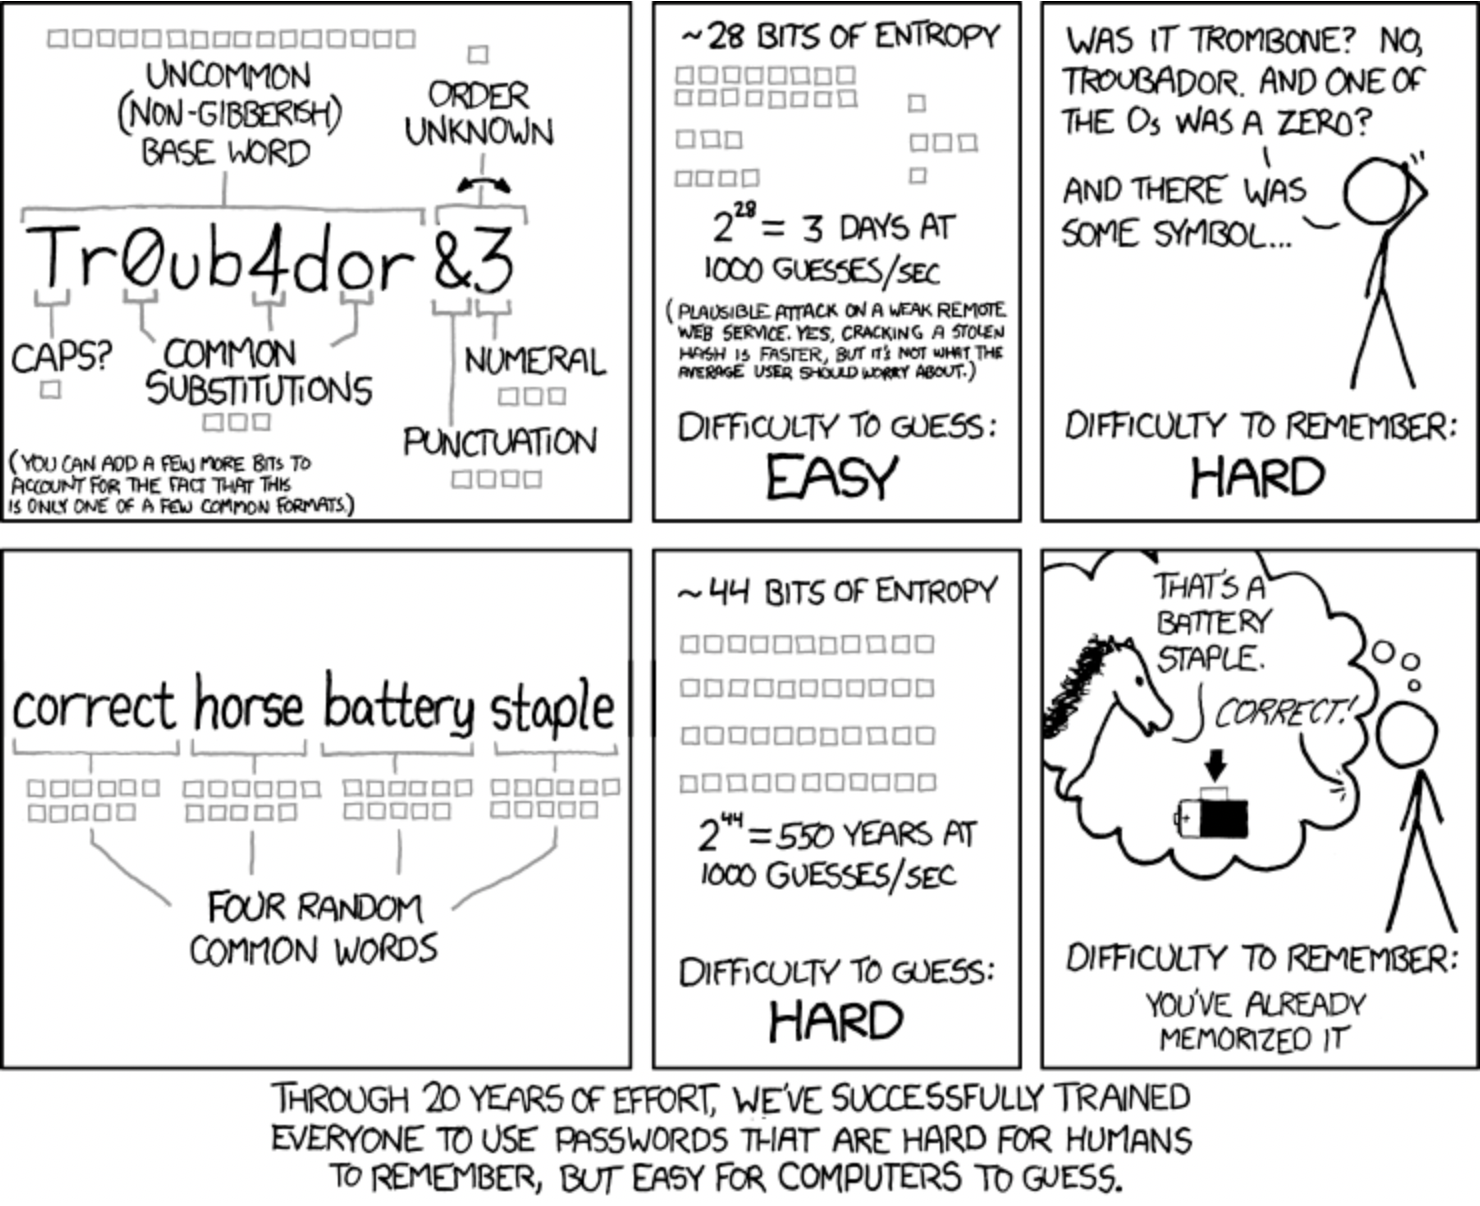
\includegraphics[width=0.5\linewidth]{xkcd/passwordStrength.png}
    \caption{\textbf{\href{https://www.explainxkcd.com/wiki/index.php/936:_Password_Strength}{936: Password Strength}}}
\end{figure}